\chapter{Suporte Tecnológico}
\label{chapter:Suporte_Tecnologico}

A fim de manter e disponibilizar o código e os artefatos gerados a partir deste trabalho, bem como o ambiente utilizado para a construção do \textit{framework}, serão apresentadas as principais ferramentas que foram utilizadas durante o seu desenvolvimento.

\section{Ferramentas de Desenvolvimento}

\subsection{Git}

Este trabalho utulizou o Git\footnote{\url{https://git-scm.com/}} (versão 1.9.1) como o sistema de controle de versão. O Git foi projetado basicamente para facilitar a vida de quem quer executar projetos em equipe de forma segura. Foi criado por Linus Torvalds, que precisava de um controle de versão rápido e que pudesse lidar com as atividades envolvidas no desenvolvimento do Kernel do Linux. Linus desejava um ferramenta livre; não encontrando, decidiu criar o Git. Esse suporte foi nomeado em referência ao próprio Linus, pois no inglês britânico, \textit{git} é uma gíria para ``cabeça-dura''.

Uma vantagem do Git é a possibilidade de controlar o projeto de forma descentralizada, ou seja, sem a exigência de um servidor mestre. A cada arquivo rastreado pelo Git, tem seu conteúdo verificado através do algoritmo de criptografia SHA-1\footnote{\url{http://www.training.com.br/lpmaia/pub_seg_cripto.htm}}.

O que faz o Git funcionar é sua habilidade de detectar mudanças em arquivos, não só que uma mudança ocorreu, mas também onde essa mudança ocorreu. Dessa forma, as alterações com problemas podem ser desfeitas, voltando para a versão estável.

\subsection{GitHub}

O GitHub\footnote{\url{https://github.com}}, lançado em 2008 e escrito em Ruby on Rails, provê um armazenamento em nuvem (\textit{Cloud}), onde se pode hospedar projetos que utilizam o Git como controle de versão. O GitHub possui funcionalidades de uma rede social como \textit{feeds}, \textit{followers}, wiki e gráficos para apresentar como os desenvolvedores trabalham em um repositório. Este lado social é interessante para descobrir novos projetos e receber ajuda em projetos particulares. É importante ressaltar que o repositório fornecido pelo GitHub é gratuito, e este repositório fica como de acesso público. Entretanto, existem planos comerciais nos quais o repositório pode se tornar privado.

A seguir é apresentada, na Figura \ref{github}, a tela de um repositório hospedado no GitHub.

\begin{figure}[!h]
	\centering
	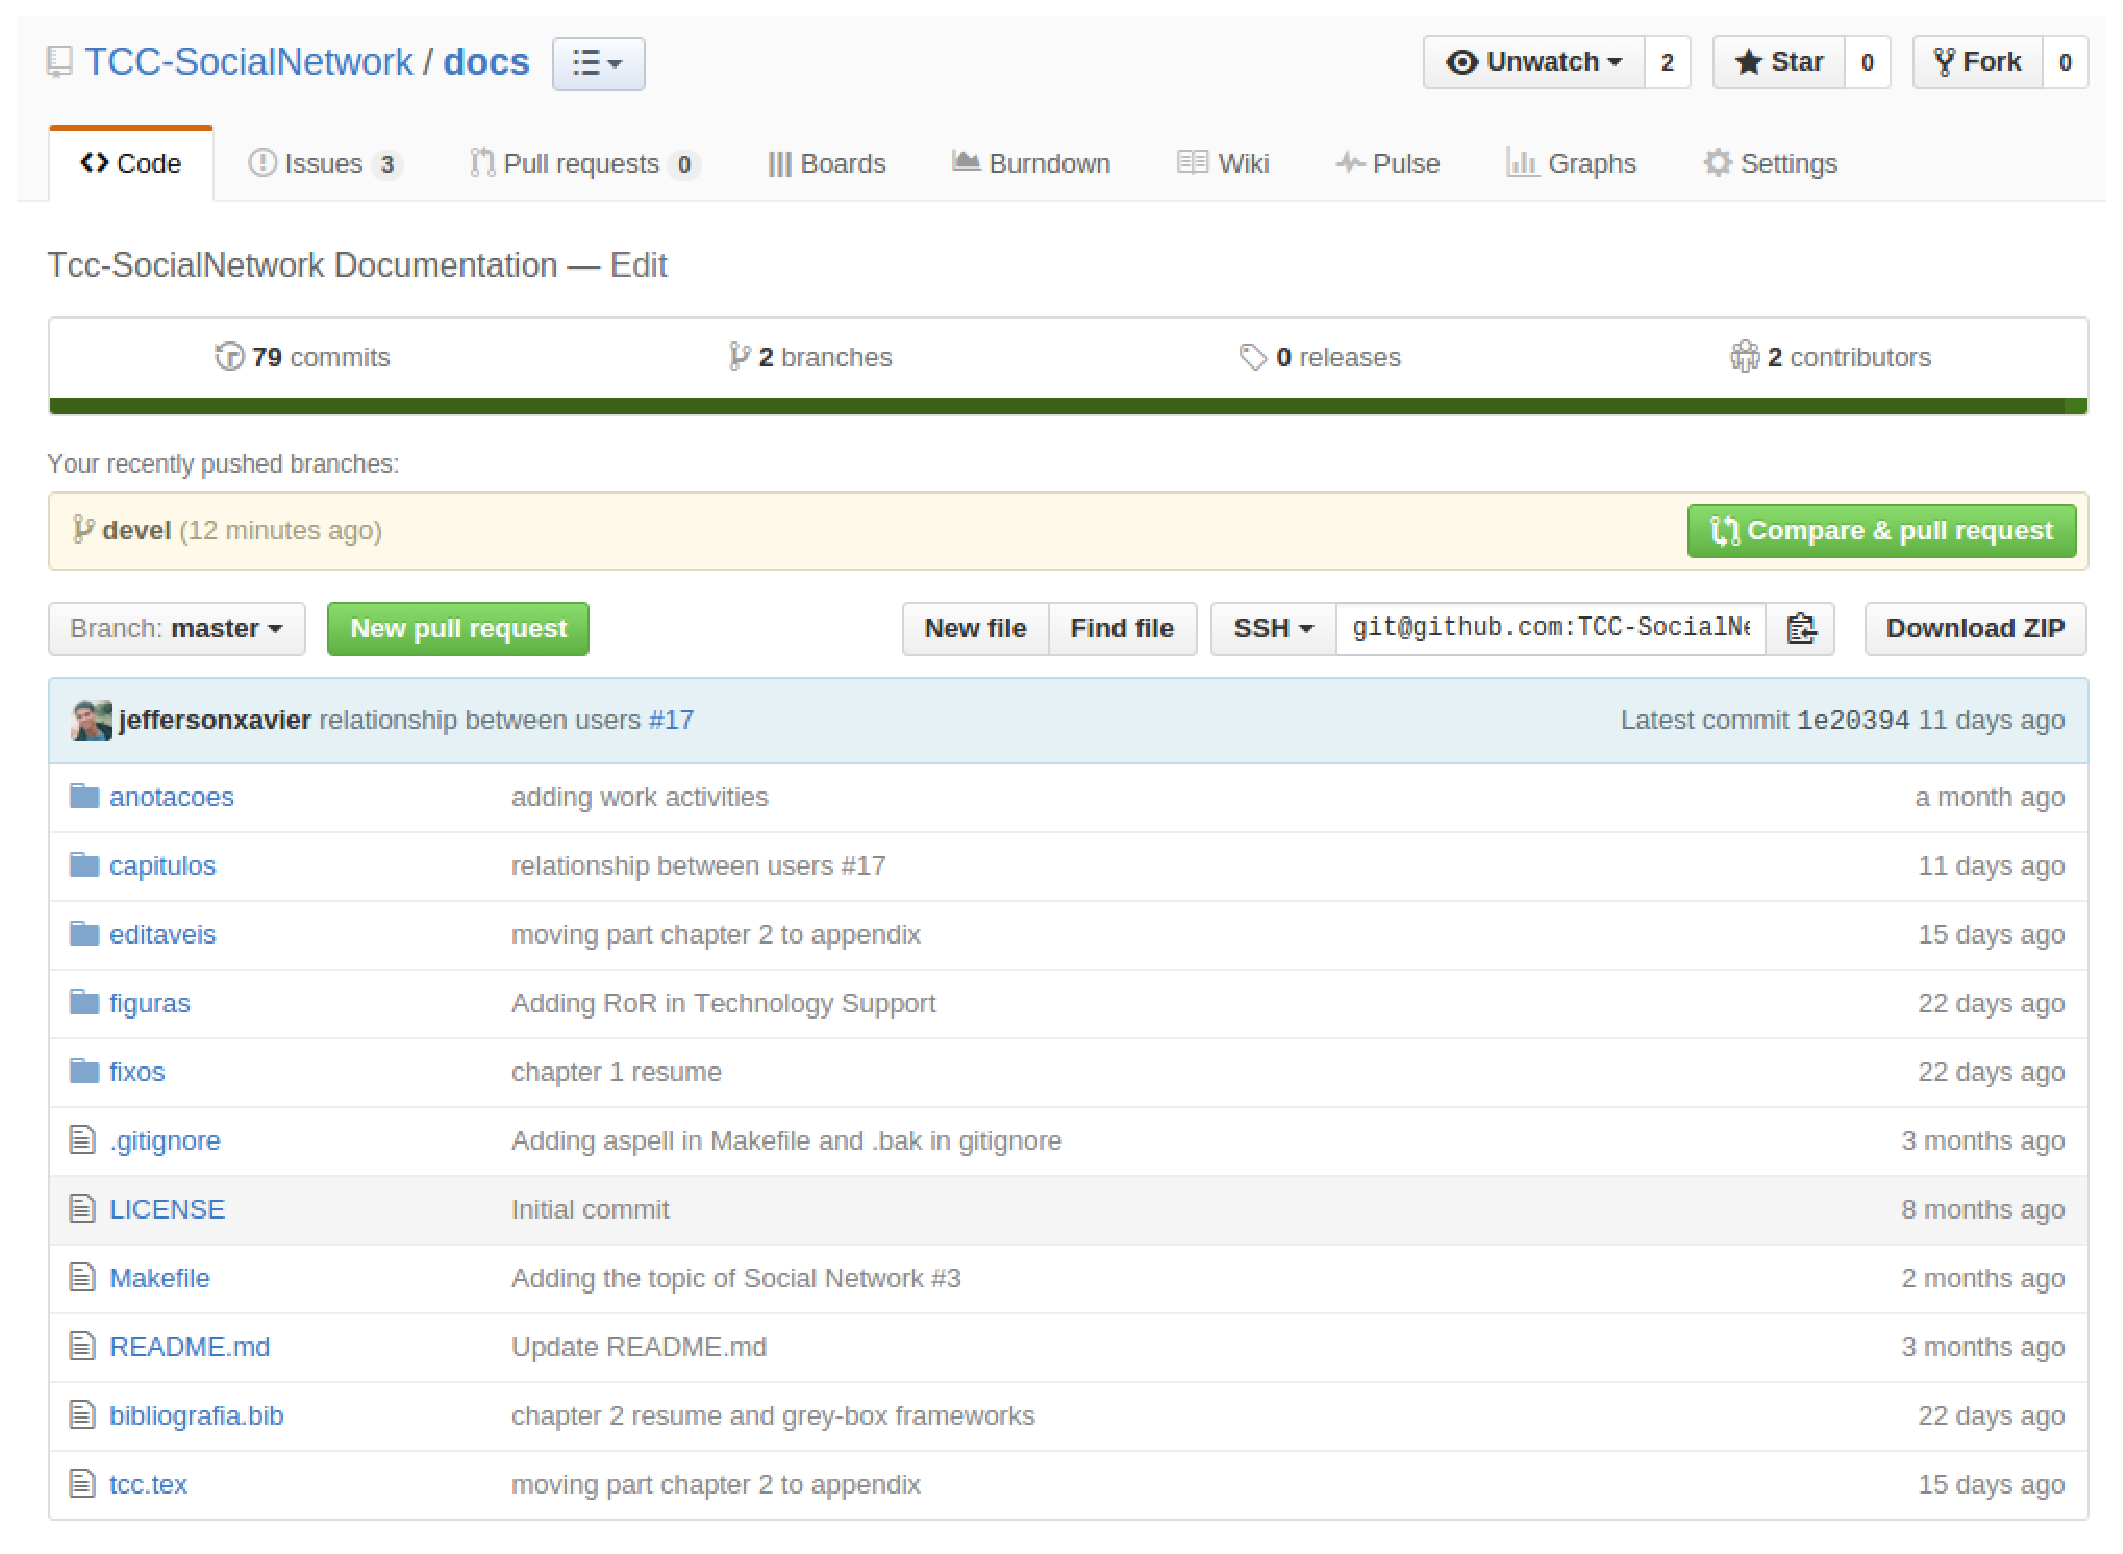
\includegraphics[scale=0.35]{figuras/suporte_tecnologico/github.eps}
	\caption{Repositório no GitHub}
	\label{github}
\end{figure}

\subsection{Waffle}

O Waffle\footnote{\url{https://waffle.io}} é um gerenciador de projetos gratuito conectado aos \textit{Pull Requests} e as \textit{Issues} do GitHub, que visa facilitar o trabalho das equipes de engenharia no que se refere ao acompanhamento das tarefas de uma forma visual, mostrando-as em um quadro com divisões para cada fase.

O Waffle escuta as ações em seu fluxo de trabalho para saber quando o trabalho é iniciado, quando está pronto para revisão, ou quando está finalizado e atualiza seu status automaticamente.

A Figura \ref{waffle} apresenta um exemplo de um \textit{board} do Waffle.

\newpage

\begin{figure}[!h]
	\centering
	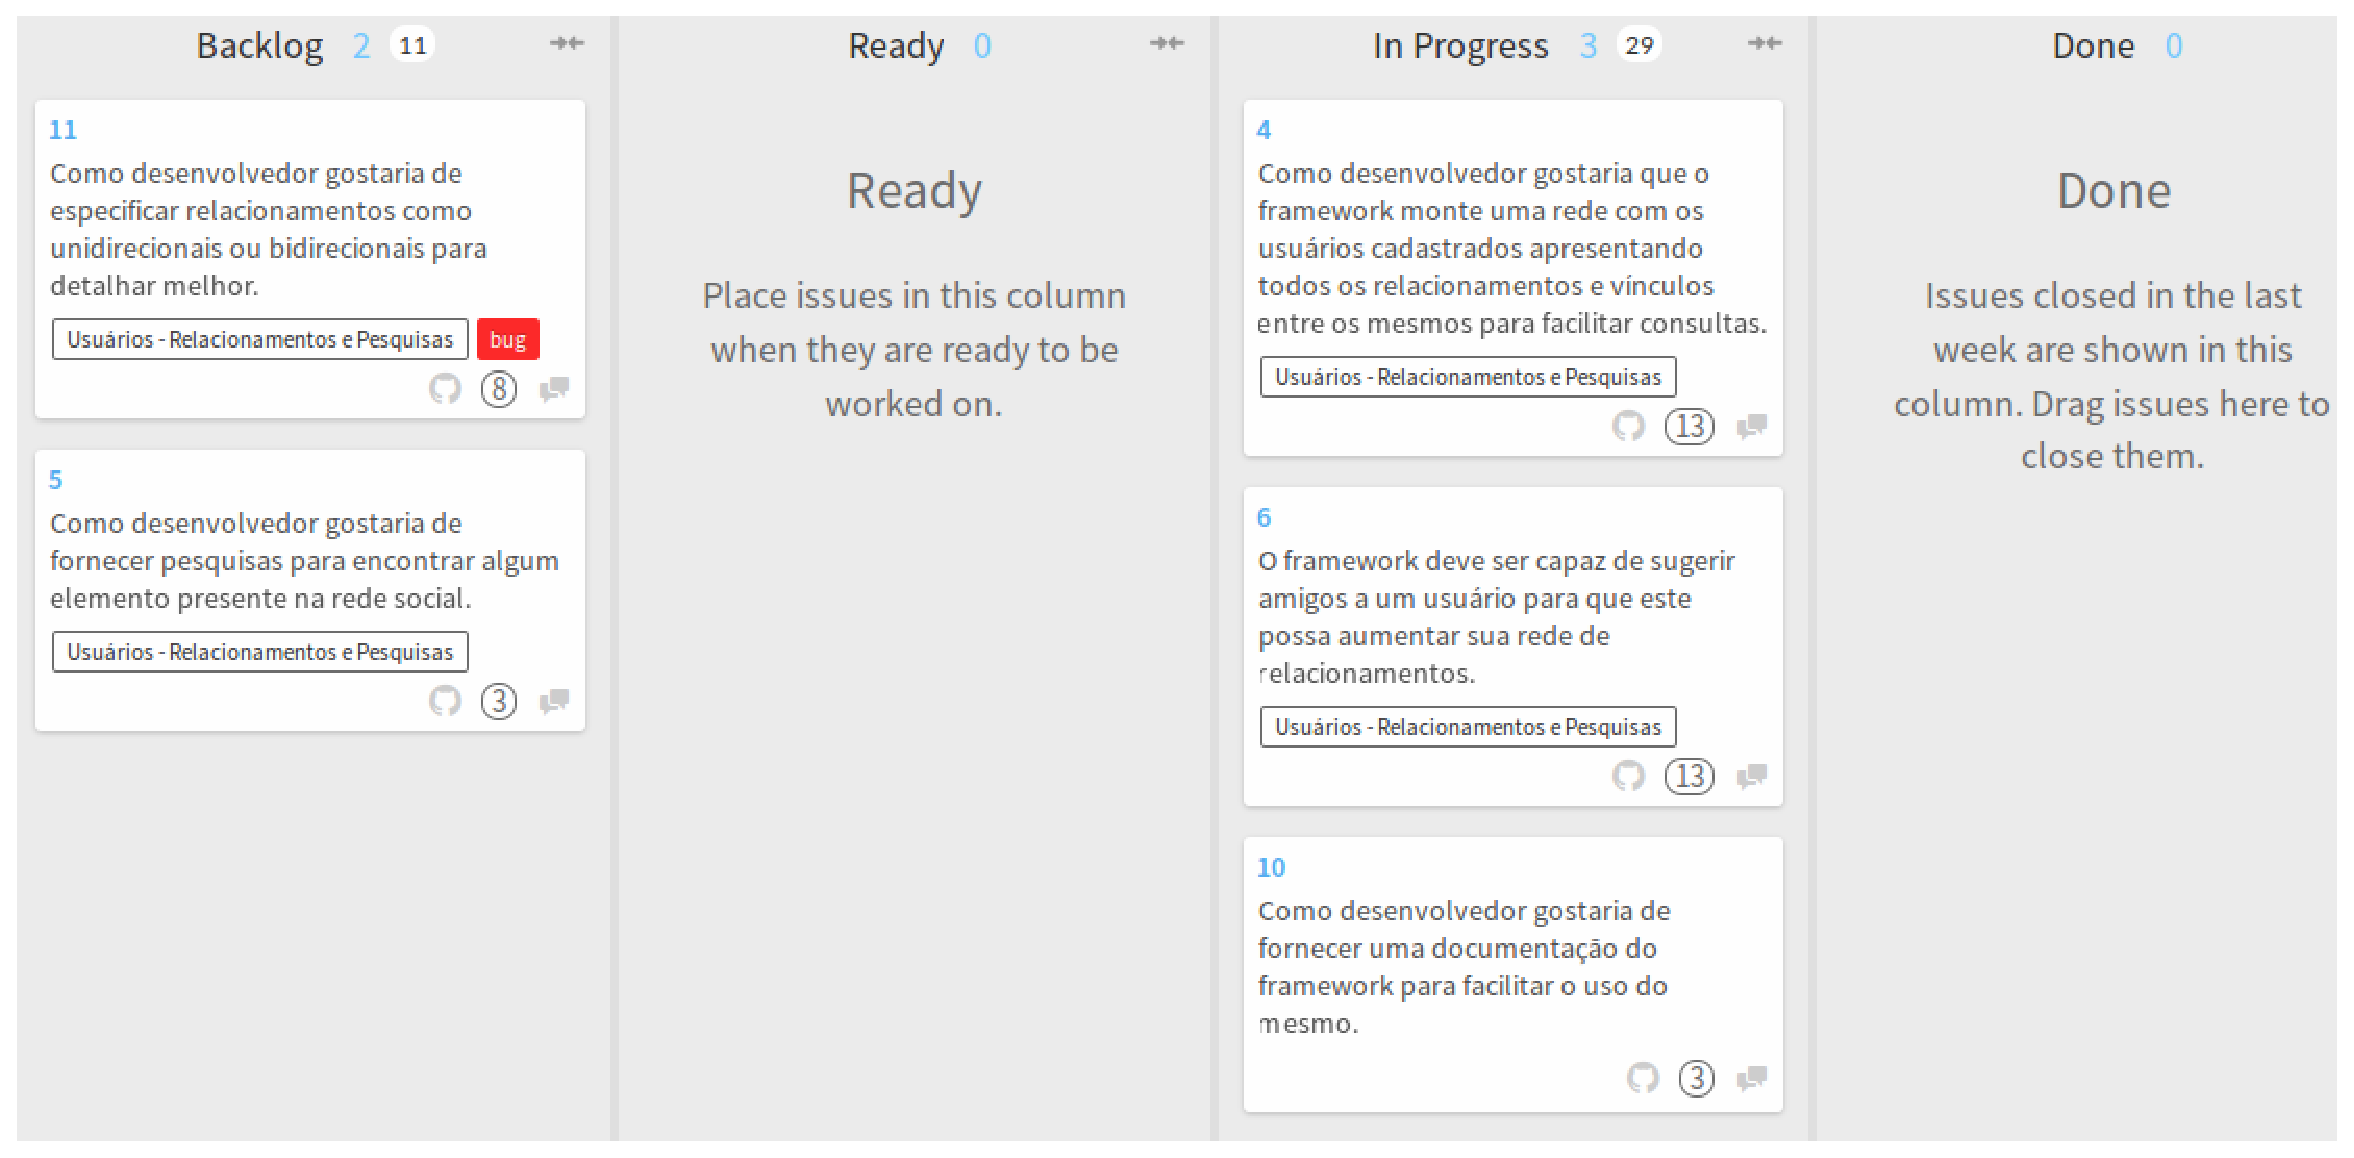
\includegraphics[scale=0.3]{figuras/suporte_tecnologico/waffle.eps}
	\caption{Board gerado pelo Waffle}
	\label{waffle}
\end{figure}

\subsection{LaTeX 3}

O \LaTeX\footnote{\url{https://www.latex-project.org}} é um pacote de macros ou marcações para o processador de textos \TeX, utilizado amplamente pela comunidade científica devido à grande qualidade tipográfica. Adicionalmente, torna mais fácil e rápida a produção de documentos em \TeX. O \LaTeX foi desenvolvido por Leslie Lamport a partir do \TeX, criado por Donald Knuth, ambos de código aberto.

O objetivo desse suporte é que o autor se distancie da apresentação visual do trabalho, concentrando-se no seu conteúdo. Para isto, ele possui formas de se lidar facilmente com estruturas como, por exemplo, bibliografias, citações, formatos de páginas e referências. O \LaTeX\ não é algo imutável, e como tal, suporta várias maneiras de estilizar e formatar os documentos.

\subsection{Sublime Text 3}

Este trabalho utilizou o Sublime Text (\textit{build 3103}) como editor de texto. Inicialmente pensado para ser uma extensão do Vim, o Sublime Text\footnote{\url{http://www.sublimetext.com/}} é um editor de texto multiplataforma, escrito em linguagem C++. Com o Sublime é possível automatizar várias tarefas a partir de recursos como, por exemplo, macros, auto-completar, repetição de ações e construção automática.

Outros recursos como dividir a tela em várias janelas, auto \textit{save}, navegação entre páginas por meio de abas e suporte a várias linguagens, por exemplo, C, C++, C\#, CSS, HTML, Java, \LaTeX, PHP, Ruby, SQL, XML, JavaScript e Groovy, fazem do Sublime uma ferramenta popular entre os programadores.

A seguir, na Figura \ref{sublime}, é apresentada uma imagem da ferramenta.

\begin{figure}[!h]
	\centering
	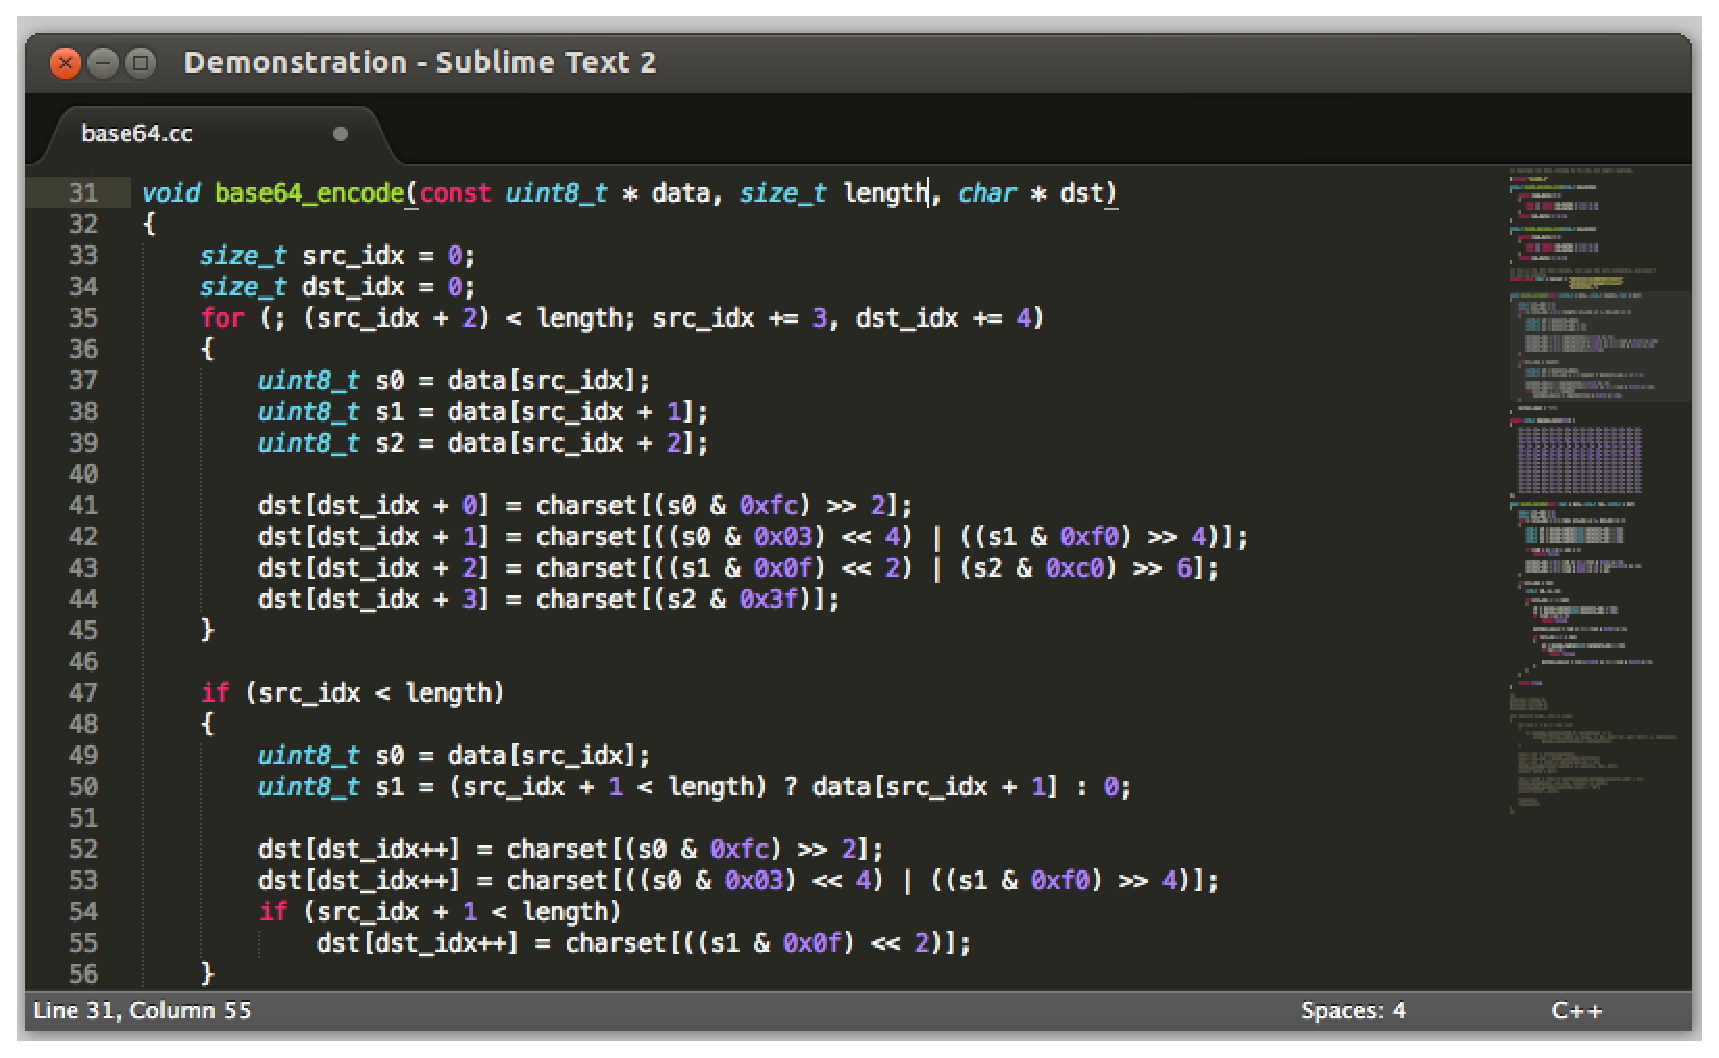
\includegraphics[scale=0.35]{figuras/suporte_tecnologico/sublime.eps}
	\caption{Sublime Text 3}
	\label{sublime}
\end{figure}

\subsection{Bizagi Modeler}

Bizagi\footnote{\url{http://www.bizagi.com}} (utilizado na versão 3.0) é uma ferramenta para modelar processos. Esta abrange tanto o mapeamento de processos de trabalho quanto a automação de processos a partir do mapeamento, permitindo que os usuários possam desenhar, documentar e compartilhar seus processos de trabalho usando a notação BPMN (\textit{Business Process Management Notation}). Um diferencial do Bizagi é a possibilidade de realizar tarefas em conjunto, utilizando um ambiente virtual.

A seguir é apresentado um exemplo de uso do Bizagi, na Figura \ref{bizagi}.

\begin{figure}[!h]
	\centering
	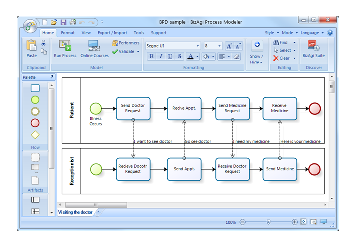
\includegraphics[scale=1.5]{figuras/suporte_tecnologico/bizagi.eps}
	\caption{Bizagi Modeler}
	\label{bizagi}
\end{figure}

\subsection{Ubuntu}

Ubuntu\footnote{\url{http://www.ubuntu.com/}} é uma palavra de origem africana que significa: ``Humanidade para os outros'' ou ainda ``Sou o que sou pelo que nós somos''. A distribuição Ubuntu traz o espírito desta palavra para o mundo do software livre. Baseado em Linux e criado a partir do Debian, o Ubuntu é patrocinado pela Canonical Ltda., e é licenciado pela licença GPL (\textit{General License Public}). Para o desenvolvimento deste trabalho foi utilizado o Ubuntu na versão 14.04 LTS.

\subsection{Ruby on Rails}

Ruby on Rails \footnote{\url{http://guides.rubyonrails.org/}} (utilizado na versão 4.2.5) é um \textit{framework} de desenvolvimento de aplicações web escrito na linguagem Ruby, projetado para tornar a programação de aplicações web mais fácil. A filosofia Rails inclui dois princípios orientadores:

\begin{itemize}
	\item \textbf{DRY} (\textit{Don't Repeat Yourself}), ou não repita a si mesmo, é um princípio de desenvolvimento de software que afirma que ``Cada pedaço de conhecimento deve ter uma única representação inequívoca e autoritária dentro de um sistema''\cite{wilson2012practices}.

	\item \textbf{Convenção sobre configuração} é um modelo onde o desenvolvedor precisa definir apenas aspectos não convencionais da aplicação e os aspectos convencionais são pré-estabelecidos. Tal estratégia evita o uso maciço de arquivos de configuração.
\end{itemize}
